\chapter{智能简史：生于数学}

\begin{introduction}
\item Definition of Theorem
\item Ask for help
\item Optimization Problem
\item Property of Cauchy Series
\item Angle of Corner
\end{introduction}

“如果人们不相信数学很简单，那是因为他们没有意识到生活有多复杂。”
\begin{flushright}
------约翰·冯·诺伊曼
\end{flushright}


智能的历史可以追溯到人类最早期的思维活动，而数学是其中最重要的基础工具之一。

对于古代人来说，数字的发明源于对数量的需求。无论是借助手指计数，还是用其他物体辅助，人类通过千年的发展，逐渐完善了从简单符号到抽象数字的演变过程。今天，我们的“自然数”概念似乎理所当然，但这一切都建立在人类历史上无数次的试错与进化中。

人类对“智能”的探讨源远流长。远在古希腊时期，哲学家们就已经开始追问：什么是智慧？什么是理性？我们如何通过思维去理解这个世界？从那时起，人们就梦想着创造能自主思考的机器。神话人物皮格马利翁(Pygmalion)、代达罗斯(Daedalus)和赫淮斯托斯(Hephaestus)可以被看作传说中的发明家，而加拉蒂亚(Galatea)、塔洛斯(Talos)和潘多拉(Pandora)则可以被视为人造生命(OvidandMartin,2004;Sparkes,1996;Tandy,1997)。

这些问题不仅关乎哲学，还对现代科学和技术的发展产生了深远影响。随着时间推移，这种对智能的追问从哲学的纯理论思辨，逐渐转向了科学与工程的实践领域。

早期的数学家如欧几里得、阿基米德以及笛卡尔等，通过逻辑和结构化的思维方式，奠定了后来发展计算机智能的理论基础。他们的工作不仅推动了科学与工程的发展，也为智能的理论构建提供了明确的框架。

\section{数字的发明，智能的开端}

\subsection{史前数学：日常需求与实用计算}
数学史往往是从公元前5世纪的希腊开始讲起的。毕达哥拉斯创立了算术，泰勒斯和阿那克西曼德创立了几何，奠定了古代数学的两大分支。算术和几何的创立，无疑是数学史上的重大突破。然而，这样的讲法却忽略了一个重要的时代，也就是所谓的“史前”数学。人们并没有等到公元前5世纪才开始解决数学问题，特别是那些日常面临的具体数学问题。

在公元前5世纪之前，数学并非一种独立的学科，而是伴随着人类生活的需要而逐步发展起来的。史前数学的主要任务是应对日常生活中的具体问题，如计数牲畜、测量土地和管理时间。远古人类通过手指计数、刻痕和结绳的方式解决了基本的数量和度量问题，虽然这些方法原始，却为后来的数学奠定了基础。

人类早期的数学成就源于实际需求，古埃及人和巴比伦人便是典型的例子。他们在天文学、土地测量和贸易中依赖数学工具，通过经验性的方法逐渐累积了丰富的数学知识。然而，这些方法主要依赖于实用性，而非系统的理论研究。

“数学”活动最古老的痕迹之一是在美索不达米亚发现的一块泥板，它可以追溯到公元前2500年。这块泥板记录了这样一个计算:如果一个谷仓里有1152000份粮食，每个人分得7份，一共可以分给多少人呢?不出所料，结果是164571人，即用1152000除以7得到的结果。看来，美索不达米亚的会计师在算术“诞生”之前很久就知道怎么做除法了。甚至，书写完全有可能就是为了记账才发明的——虽然这些事情很难说得准，但若真是如此，数字就比字母发明得还要早了。

\subsubsection{手指：长在身上的计数器}
相信你在许多影视剧中都见过这样的一幕：一位算命先生，掐指一算，口中念念有词。这种“掐指一算”看似神秘，实则源自于古老而简便的计数方法。
\begin{figure}[htbp]
\centering
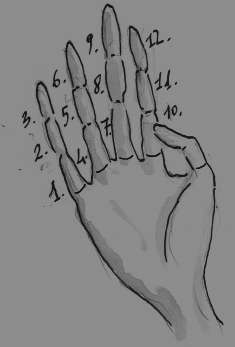
\includegraphics[width=0.5\textwidth]{figs/fingers.png}
\caption{“掐指一算”}
%\label{}
\end{figure}

在远古时代，用手指计数是再自然不过的选择，手指是人类最早的“随身计算器”。手指提供了一个天然的计数系统，帮助人们轻松应对日常的计数需求，如记录牲畜数量、物品交换量，推算季节、节气，安排农耕节日等活动。

%\subsection{手指计数与各种进制系统}
手指的构造与多种进制系统有着天然的联系。稍加思考，我们就可以发现十进制、二十进制、十二进制等计数法与手指构造的对应关系。

十进制(Decimal System)是最常见、最自然的计数方式。双手的十根手指与十进制自然对应，每根手指代表一个数字，从1数到10，完成一轮计数。十进制系统在全球的广泛使用，源于人类天生拥有十根手指的解剖学特征。正如爱德华·卢卡斯所言，这是“自然界的一个偶然事件”​。

十二进制(Duodecimal System)则适用于更复杂的计数需求。除大拇指外，四根手指各有三段指节。一只手的大拇指指向四根手指的各段指节，可以计数1到12。这种方式在古代美索不达米亚和古埃及广泛应用，至今仍用于时间和角度的计数系统中，如12小时制、一年12个月等。

六十进制(Sexagesimal System)则更加复杂。它结合双手来计数。一只手用于计12（与十二进制相同），另一只手的五根手指则记录12的倍数，五轮12等于60。六十进制在古巴比伦时期被发明，沿用至今，广泛用于时间和角度的计量，例如1小时=60分钟，1分钟=60秒，以及360度的圆周划分。

二十进制(Vigesimal System)也是一种古老的计数法。为了更大范围的计算，一些古代民族不仅用手指，还加上脚趾来计数。例如，中美洲的玛雅文明和阿兹特克文明，以及现今的西非和欧洲部分地区，采用了以20为基数的计数法。

二十进制的痕迹在许多语言中依然存在。现代英语中的"score"表示20的用法便保留了这一印记。例如，莎士比亚在《圣经》英译本中使用“three score and ten”（20的3倍加10，表示70岁)来指代古稀之年；林肯在《葛底斯堡演讲》中使用“four score and seven years ago”(20的4倍加7，表示87)来表达87年前的历史。一百年后，马丁·路德·金在其著名的演讲《I have a dream》中说“Five score years ago”​（20的5倍，即100年前）​。如今，在现代英语中，“score”的这种用法已不再常见。

英国曾有一个结合十二进制和二十进制的货币系统：1英镑=20先令，1先令=12便士。1971年，英国引入了十进制货币系统，1英镑=100便士，先令在1990年后彻底退出流通。

在法语、丹麦语和巴斯克语中也能找到二十进制的痕迹。例如，法语中的数词从quatre-vingts(80)​、quatre-vingts-dix(90)​，到quatre-vingts-dix-neuf(99)，表明凯尔特族过去采用二十进制计数法。同时，这些语言中还混杂了六十进制的痕迹，如数词soixante(60)到soixante-dix-neuf(79)。

手指不仅是我们身体的一部分，还是人类最早的天然计算工具。它帮助我们理解和组织世界，并为现代数学中的位值制和进制系统提供了最初的灵感。直到今天，手指仍是许多人在进行简单计算时的本能工具。可以说，手指是人类最早的“计算器”，引领我们从最原始的计数方法走向了复杂的数学世界。

\subsection{自然的教育，数字文明的缩影}
设想你在一次航海探险中遭遇风暴，不幸漂流到了一个无人孤岛。没有手表、手机，也没有任何现代工具。你很快面临一个问题——如何计算时间？如何记录每天收集的食物？在这种完全回归自然的环境中，你必须依靠最原始的方式来解决这些问题。

\subsubsection{手指计数：最简单的工具}
你的第一反应可能是是用手指来计数。十根手指天生就是人类最便捷的“计算器”，帮助你快速记录简单的数量——比如你捕到的鱼或采摘的果实。手指计数是直观而方便，几乎无需思考就能完成。但很快，你意识到这种方法有明显的局限性：当数字变大，或需要记录更复杂的信息时，手指显然不够用了。更重要的是，手指计数无法保存这些数据，一旦忘记，你的记录便随之消失。

\subsubsection{刻痕计数：更长久的记录方式}
为了更长久地保存记录，你开始在岛上的树木或石头上刻下痕迹。每道刻痕代表一天的过去，或你每天捕获的鱼或采摘的果实数量......。刻痕计数法让你能够更长久地保存这些信息。每天的刻痕不断累积，形成一个记录时间和活动的系统。这种方法虽然简单，却比手指计数更加持久、可靠，也能应对稍微复杂的需求，比如记录日期或特定的事件。然而，随着时间的推移，刻痕的数量增加，管理这些信息变得越来越困难。你开始需要一种更便捷、更灵活的方式来记录和传递这些信息。

\subsubsection{结绳记数：更高级的记数法}
幸运的是，你发现了一根绳子，这给了你一个新的选择——结绳记数法。通过在绳子上打不同的结，你可以标记不同的天数、事件或物品的数量。不同形状和位置的结可以表示不同的信息。相比于刻痕，结绳计数法更便捷灵活，更易于携带和传递，成为你在荒岛生活中的高级计数工具。

\subsubsection{荒岛上的自然教育：人类数字发明的倒影}
在这场荒岛冒险中，随着你逐步探索各种计数方法，你无意间接受了一种独特的自然教育。这个经历，其实正是早期人类如何发明和发展数字的缩影。在远古时代，人类也像你一样，从最初的手指计数，逐渐发展到刻痕和结绳，寻找更有效的计数方式，逐渐探索出了越来越复杂、抽象的记数方式。

你在荒岛上的探索，正是人类数字文明进化的缩影。无论是刻痕还是结绳，这些方法都体现了人类从最初的物理标记到复杂符号系统的演化路径。通过这些自然的计数方法，你逐步掌握了记录、比较和计算的基本概念。这不仅是你个人的“自然教育”，也是数字发明的最初动力——让生活更加便捷和高效。

\subsection{数字的位值系统}
在人类早期文明中，简单的手指计数和结绳、刻痕等计数方法已广泛用于记录数字，帮助人们应对日常的数值计算。然而，随着社会的发展，人们逐渐认识到，仅靠刻痕和结绳等物理标记在处理更复杂和更大范围的数字时，显得低效而繁琐。 于是，更加抽象的符号系统应运而生。从而催生了{\bf 位值制}这一革命性的数字表示方式,使得复杂的数值能够通过简单的符号位置来表示和计算。

早期的计数系统大多采用{\bf 加法规则}。例如，在古代巴比伦的黏土板上，数字是通过符号的重复来表示的：数字“1”用一个符号表示，数字“2”用两个相同符号表示，数字“3”则用三个相同符号。
这种计数方式很眼熟，中文数字、罗马数字、古印度的婆罗门数字和笈多王朝使用的数字，以及大洋彼岸的玛雅数字，都采取了同样的方法。大多数的古代文明在表示前三个数字时，都采取了同样的方式：重复表示“1”的符号一次，两次，三次。古代的中文“一、二、三”、钟表盘上的罗马数字“Ⅰ、Ⅱ、Ⅲ”、阿拉伯数字也体现了同样的重复方式。可是，从数字4开始，所有的文明就都放弃了这种重复。为什么呢？

研究发现，人类的数感对少于3的数字有天然的反应，但超出这个范围后，单纯的重复符号便变得困难。对一些出生几个月的婴孩进行试验，结果证实人类与生俱来的数感的容量不超过三。

试想一下，数字13若用重复排列“1”的符号13次来表示，无论是对书写还是阅读，都会很低效---怎么能一眼就看出它是13，而不是12或者14呢？

类似的问题在罗马数字系统中也很常见。罗马数字系统中，V表示5，X表示10，L表示50，C表示100。此外，向右添加符号为加，如，VI表示数字6，XI表示数字11；相反地，向左添加一个更小数值的符号为减，如IV表示4，IX表示9。
尽管使用了加减法规则的计数系统十分直观，但在表示大数时显得十分低效。例如1888年写成罗马数字就是MDCCCLXXXVIII，甚至无法有效表示类似100万那样的数字——除非把1000个M排成一排!

随着人类文明的发展，许多地区开始引入更为先进的计数法，其中最具革命性的是{\bf 位值制计数法}。古巴比伦、中国，尤其是印度和阿拉伯，率先采用了这种创新的位值制计数法。
这种计数法的关键在于符号的位置决定了其数值。例如，数字“12”和“21”虽然使用相同的符号，但因为符号位置不同，代表的数值也不同。

位值计数法具有出众的简洁性。
通过有限的符号，可以表达任意大的数值。
例如，$10^{100}$这个超出了物理限制的天文数字，在位值制下仅需101个符号即可表示——一个"1"后面跟着100个"0"。位值计数法用极短的符号链表示极其巨大的数值。

位值制不仅提高了数字的表示效率，还反映了数字的{\bf 对数增长}特性，即随着数字的增大，所需的符号长度呈对数增长，符号数量远远少于数字本身的大小。例如，表达$10^{100}$所需的符号长度约为$log_10 10^{100}=100$ (实际为101个)。
一般地，表达任意整数 $x$所需的符号数量接近$log_{10} x$。
因此，从某种意义上，位值计数系统是最简洁、甚至最优的。

位值制的引入是人类计数方法的一次重大飞跃。从简单的重复符号到高度抽象的符号系统，位值制极大简化了计算过程，推动了计算和数学的发展，奠定了现代数字系统的基础。

\subsection{位值制与对数增长在现代计算机中的应用}
在计算机科学中，在已经排好序的数组中查找某个元素的时间也是数组长度的对数。即使数组规模如同宇宙般庞大，经过几百次迭代后，便能够找到所需的元素——唯一的限制就是光速有限性所带来的信息传播和处理速度的物理极限。

互联网的URL是位值制与对数增长在数据处理和网络寻址中的一个典型应用。一个简短的URL(Uniform Resource Locator，URL，统一资源定位符)迅速定位到海量信息。
想象一下，你希望在网上搜索某项信息。尽管互联网上的数据量可能以EB($10^{18}$字节)甚至ZB($10^{21}$字节)计量，只要拥有对应信息的URL，你几乎瞬间就能找到目标信息。
这正是对数增长的强大之处：即使面对巨大规模的数据集，只需少量步骤就能完成检索。

此外，URL的简短程度令人惊叹，其长度是整个网络大小的对数！这意味着我们可以轻松将URL存储在内存中，而URL指向的信息量却远远超出了其自身长度。
这种简洁有效的特性，展示了对数增长在计算与信息处理中的关键作用。

IPv4和IPv6的设计正是对数增长在实际应用中的另一个实例。
 IPv4地址使用{\bf 32位}二进制数来表示，每个IP地址可以被写成4个以点分隔的十进制数（如192.168.1.1），每部分对应一个8位的二进制数。
32位的二进制能够生成$2^{32}$，即约{\bf 43亿}个唯一IP地址。这在IPv4设计之初被认为是足够庞大的数目。然而，随着互联网的迅速扩展，特别是物联网（IoT）设备和移动设备的广泛普及后，IPv4的43亿个地址空间将很快耗尽。

   为了解决这一问题，{\bf IPv6}应运而生。IPv6使用{\bf 128位}二进制数表示，由八组以冒号分隔的16进制数构成(如 2001:0db8:85a3:0000:0000:8a2e:0370:7334)。这种128位的二进制表示能生成$2^{128}$，即约{\bf $3.4 \times 10^{38} $} 个唯一IP地址，相当于为地球上的每粒沙子分配多个IP地址。这一数量级足以应对未来几十年甚至几百年内所有联网设备的需求。
   
IPv4和IPv6的位数与它们能够支持的地址数量之间的巨大落差，展示了对数增长的强大力量。IPv4仅用32位符号就能表示43亿个地址，而IPv6仅用128位符号就能支持{\bf $3.4 \times 10^{38}$}个地址。随着位数的增加，IP地址系统实现了指数级的扩展，同时保持了地址表示的简洁性。

%再那些颠覆时代的宿命时刻中扮演重要角色的任务，如毕达哥拉斯，带有强烈的传奇色彩。他们埋头钻研不可能的问题，如化圆为方。他们将自己的才智倾注于探索数学的奥秘，创造了思维中的世界，并在其中找到了可以真实描述现代“宇宙工厂”的表达方式。不必借助幻想去解释这些宿命时刻的诞生，因为，正如茨威格所说，在那些超凡的时刻，“历史不需要帮助”。

\section{数字：从具象到抽象}
几千年来，人类都在探索如何建立数与物的对应关系，现代数字系统的定义正是基于这种探索的延续。一旦人类掌握了计数，数字系统的应用就变得“自然而然”了。或许正因如此，我们才称自然数为“自然”数(natural number)。然而，实际上，数字的概念一点也不“自然”。

无论是在早期人类在骨头及木棍上有序地刻下划痕，还是结绳或是在容器中放置物品无论是结绳，这些早期方法已代表了相当抽象的符号系统，其中抽象的数学对象与自然中的实际物体之间的分离，同一个数字既可以表示动物的数量，也可以记录借贷量或一个月的天数。
自此之后，数学研究的对象不再是必须与实际物体相关的几何图形和数字。研究对象性质的变化，最终引发了解决数学问题的方法的革命。

\section{数学的真正诞生：从计算到推理}
%\subsection{从实用到抽象}
数学作为一种学科，经历了漫长的演化过程。起初，数学的诞生是为了解决生活中的实际问题——如何计数、测量、交易、管理时间等。

公元前5世纪的希腊是数学发展的转折点。在此之前，数学主要集中于如何进行计算。

在埃及和美索不达米亚等古老文明中，数学的发展更多地依赖于经验和实际操作。埃及的数学侧重于土地测量、建筑工程和会计管理，而巴比伦人则在天文学、时间计算和度量衡方面取得了显著的成就。他们的数学面向解决日常问题，更多依赖于表格、算法和简单的数值操作。

“数学”活动最古老的痕迹之一是在美索不达米亚发现的一块泥板，它可以追溯到公元前 2500 年。这块泥板记录了这样一个问题：一个谷仓里有 1152000 份粮食。如果每个人分得7份，一共可以分给多少人？答案是 164571人，即用 1152000 除以7得到的结果。看来，美索不达米亚的会计师在算术“诞生”之前很久就知道怎么做除法了。美索不达米亚和埃及的会计师不仅会做乘除法，而且掌握了许多其它的运算，比如解二次方程等。土地测量师则会计算矩形、三角形、圆形的面积。

这种实用性的数学(包括算术和几何)在数学史上称为“史前”数学，因为它并不涉及抽象推理，而是围绕日常需求展开。
	
因此，教科书中的数学史往往是从公元前5世纪的希腊开始讲起的，因为希腊数学家让数学从“如何计算”进化到了“为什么如此”。

在公元前5世纪的希腊，毕达哥拉斯学派提出了这样一个问题：找出一个等腰直角三角形，使其三边的长度都是自然数。
假设等腰直角三角形的直角边长度为$x$，斜边长度为$y$。根据毕达哥拉斯定理(勾股定理), ~$y^2$ 就等于~$x^2+x^2$。因此，这个问题最终归结为：找出两个自然数$x$和$y$，使得
\begin{equation}\label{eqn}
2x^2=y^2。
\end{equation}
让我们来试试4以内所有x和y的可能性吧 (见表~\ref{tab:example})。
\begin{table}[htbp]
\centering
\begin{tabular}{|c|c|c|c|}
\hline
$x$ & $y$ & $2x^2$ & $y^2$ \\
\hline
1 & 1 & 2 & 1 \\
\hline
1 & 2 & 2 & 4 \\
\hline
1 & 3 & 2 & 9 \\
\hline
1 & 4 & 2 & 16 \\
\hline
2 & 1 & 8 & 1 \\
\hline
2 & 2 & 8 & 4 \\
\hline
2 & 3 & 8 & 9 \\
\hline
2 & 4 & 8 & 16 \\
\hline
3 & 1 & 18 & 1 \\
\hline
3 & 2 & 18 & 4 \\
\hline
3 & 3 & 18 & 9 \\
\hline
3 & 4 & 18 & 16 \\
\hline
4 & 1 & 32 & 1 \\
\hline
4 & 2 & 32 & 4 \\
\hline
4 & 3 & 32 & 9 \\
\hline
4 & 4 & 32 & 16 \\
\hline
\end{tabular}
\caption{4以内$x$与$y$的所有可能性}
\label{tab:example}
\end{table}
在上述所有情况里，$2x^2$ 都不等于$y^2$。我们当然还可以在更大的数字范围里继续寻找。事实上，毕达哥拉斯学派很可能寻找了很久，却没能找到解。后来，他们终于相信这个解不存在。他们是怎么说服自己这个解不 存在的呢?显然不是穷尽所有的数对，因为这样的数对有无穷不可数个。你就算试到 1000 甚至 100 万 ，证实没有数对能满足条件，可你还是没法保证在更大的数字里面不可能有解......

既然不能用穷举法，那就试试逻辑推理。 
不妨假设$x,y$两个数互素。为什么呢？因为若$x,y$至少有一个是奇数时，两者自然互素；反之，若$x,y$都是偶数，则总是可以通过消去公因子来保证$x,y$至少有一个是奇数。
据此，我们把数对$x,y$分成以下3种情况: 
\begin{enumerate}
\item $x,y$都是奇数;
\item $x$是偶数，$y$是奇数;
\item $x$是奇数，$y$是偶数;
%\item $x,y$都是偶数。
\end{enumerate}

我们先从第一种情况开始：$x$ 和 $y$ 都是奇数。此时~\eqref{eqn}的解不存在。因为 $y$ 是奇数，则$y^2$也是奇数。它不可能等于$2x^2$，因为后者必然是偶数。这一论证也同样适用于第二种情况，即 $x$ 是偶数而 $y$ 是奇数。第三种情况即 $x$ 是奇数而 $y$ 是偶数。但在这种情况下，若$2x^2=y^2$成立，则这个数的一半$x^2$ 是奇数，同时$y^2$的一半却是偶数——这两个数不可能相等。
综上所述，找不到两个自然数$x,y$ 满足~\eqref{eqn}。

为了证明这个问题没有解，毕达哥拉斯学派采用了逻辑推理而不是计算来实现。他们通过分类讨论和推理，证明了无论 $x$ 和 $y$ 是奇数还是偶数，方程 $2x^2 = y^2$ 都不可能有整数解。


这一问题的解决在数学史的发展上具有划时代的意义。它的革命性不仅在于其对未来数学的巨大影响，还在于其抽象性及解决的方法。相比于美索不达米亚泥板上铭刻的诸如“将1152000份粮食除以7份”的具体问题，毕达哥拉斯学派的问题更为抽象：美索不达米亚的会计师关注粮食的数量，而毕达哥拉斯学派的问题仅涉及数字本身。同样，他们处理的是抽象的几何形式，而非具体的三角形田地。从从粮食的份数到数字，从实际的土地测量转向几何学的抽象思考，迈向抽象这一步的意义不可小觑。田地的面积无非几平方千米，而抽象的几何对象则可以轻松超越这一尺度，进入无限的范围。

古希腊数学家不再满足于计算结果，而是开始重视推导过程。他们通过严谨的逻辑推理，逐步构建了数学证明和公理系统。
这一从计算到推理的转变，被视为数学的真正诞生，使得数学从日常的计算工具演变为以推理和抽象为核心、具有高度抽象和严谨逻辑的独立学科的学科。

一个平方数不可能是另外一个平方数的两倍——这个由毕达哥拉斯学派 在 2500 多年前得到的结果，迄今在数学上仍占有重要地位。它证明了，一个短边为 1 米的等腰直角三角形中，斜边的长度为$\sqrt{2}$，约 1.414，但这个数无法通过两个自然数 $y$ 和 $x$ 的比值得到。这揭示了，某些几何关系无法通过自然数的四则运算(加、减、乘、除)运算得到，暗示了更广泛的数系——实数的存在。这一发现让数学进入了一个全新的领域——从实际问题中抽象出纯粹的数学对象并通过推理得出结论。
虽然这一发现具有革命性，但毕达哥拉斯学派并没有进一步发展出实数的概念。对他们而言，这一结论动摇了他们对自然数“万物皆数”的信仰，甚至引发了哲学上的困惑与争议。然而，几百年后，这一发现启发了数学家们发展出实数理论，为数论和分析学的诞生奠定了基础。

在古希腊，%数学从计算工具发展成为推理科学，
算术与几何逐渐成为两大数学分支。毕达哥拉斯创立了算术，泰勒斯和阿那克西曼德奠定了几何的基础。这两个分支的诞生，标志着数学从实用计算工具演变为一门以逻辑推理和证明为核心的科学。古希腊数学家的工作不仅为现代数学的发展铺平了道路，也为整个科学体系奠定了坚实的理论基础，开启了数学从经验工具到推理科学的伟大飞跃。

\newpage
